
\subsection{Study Design}
\label{sec:study-design}

The main purpose of the study was to understand people’s qualitative
perceptions of monitoring in the workplace. We used semi-structured
interviews and focus groups to explore individual perspectives. 
Interviews and focus groups were structured around three main
questions:

\begin{enumerate}
\item What are occupants’ perceptions of occupancy monitoring in their workplace?
\item How would occupants’ perceptions of occupancy monitoring change
  (or not) if they were engaged in a process of identifying key
  building issues that monitoring could help resolve and exploring
  scenarios of how that could happen? 
\item What do occupants want from monitoring?
\end{enumerate}

We used a simple data visualisation to show people what data was being
collected as well as a sample day’s data. This is illustrated in
figure~\ref{fig:dataviz}.\footnote{
An online version of the visualization can be found at \url{http://www.aviz.fr/~bbach/occupancy/}.
}

\begin{figure}
  \centering
  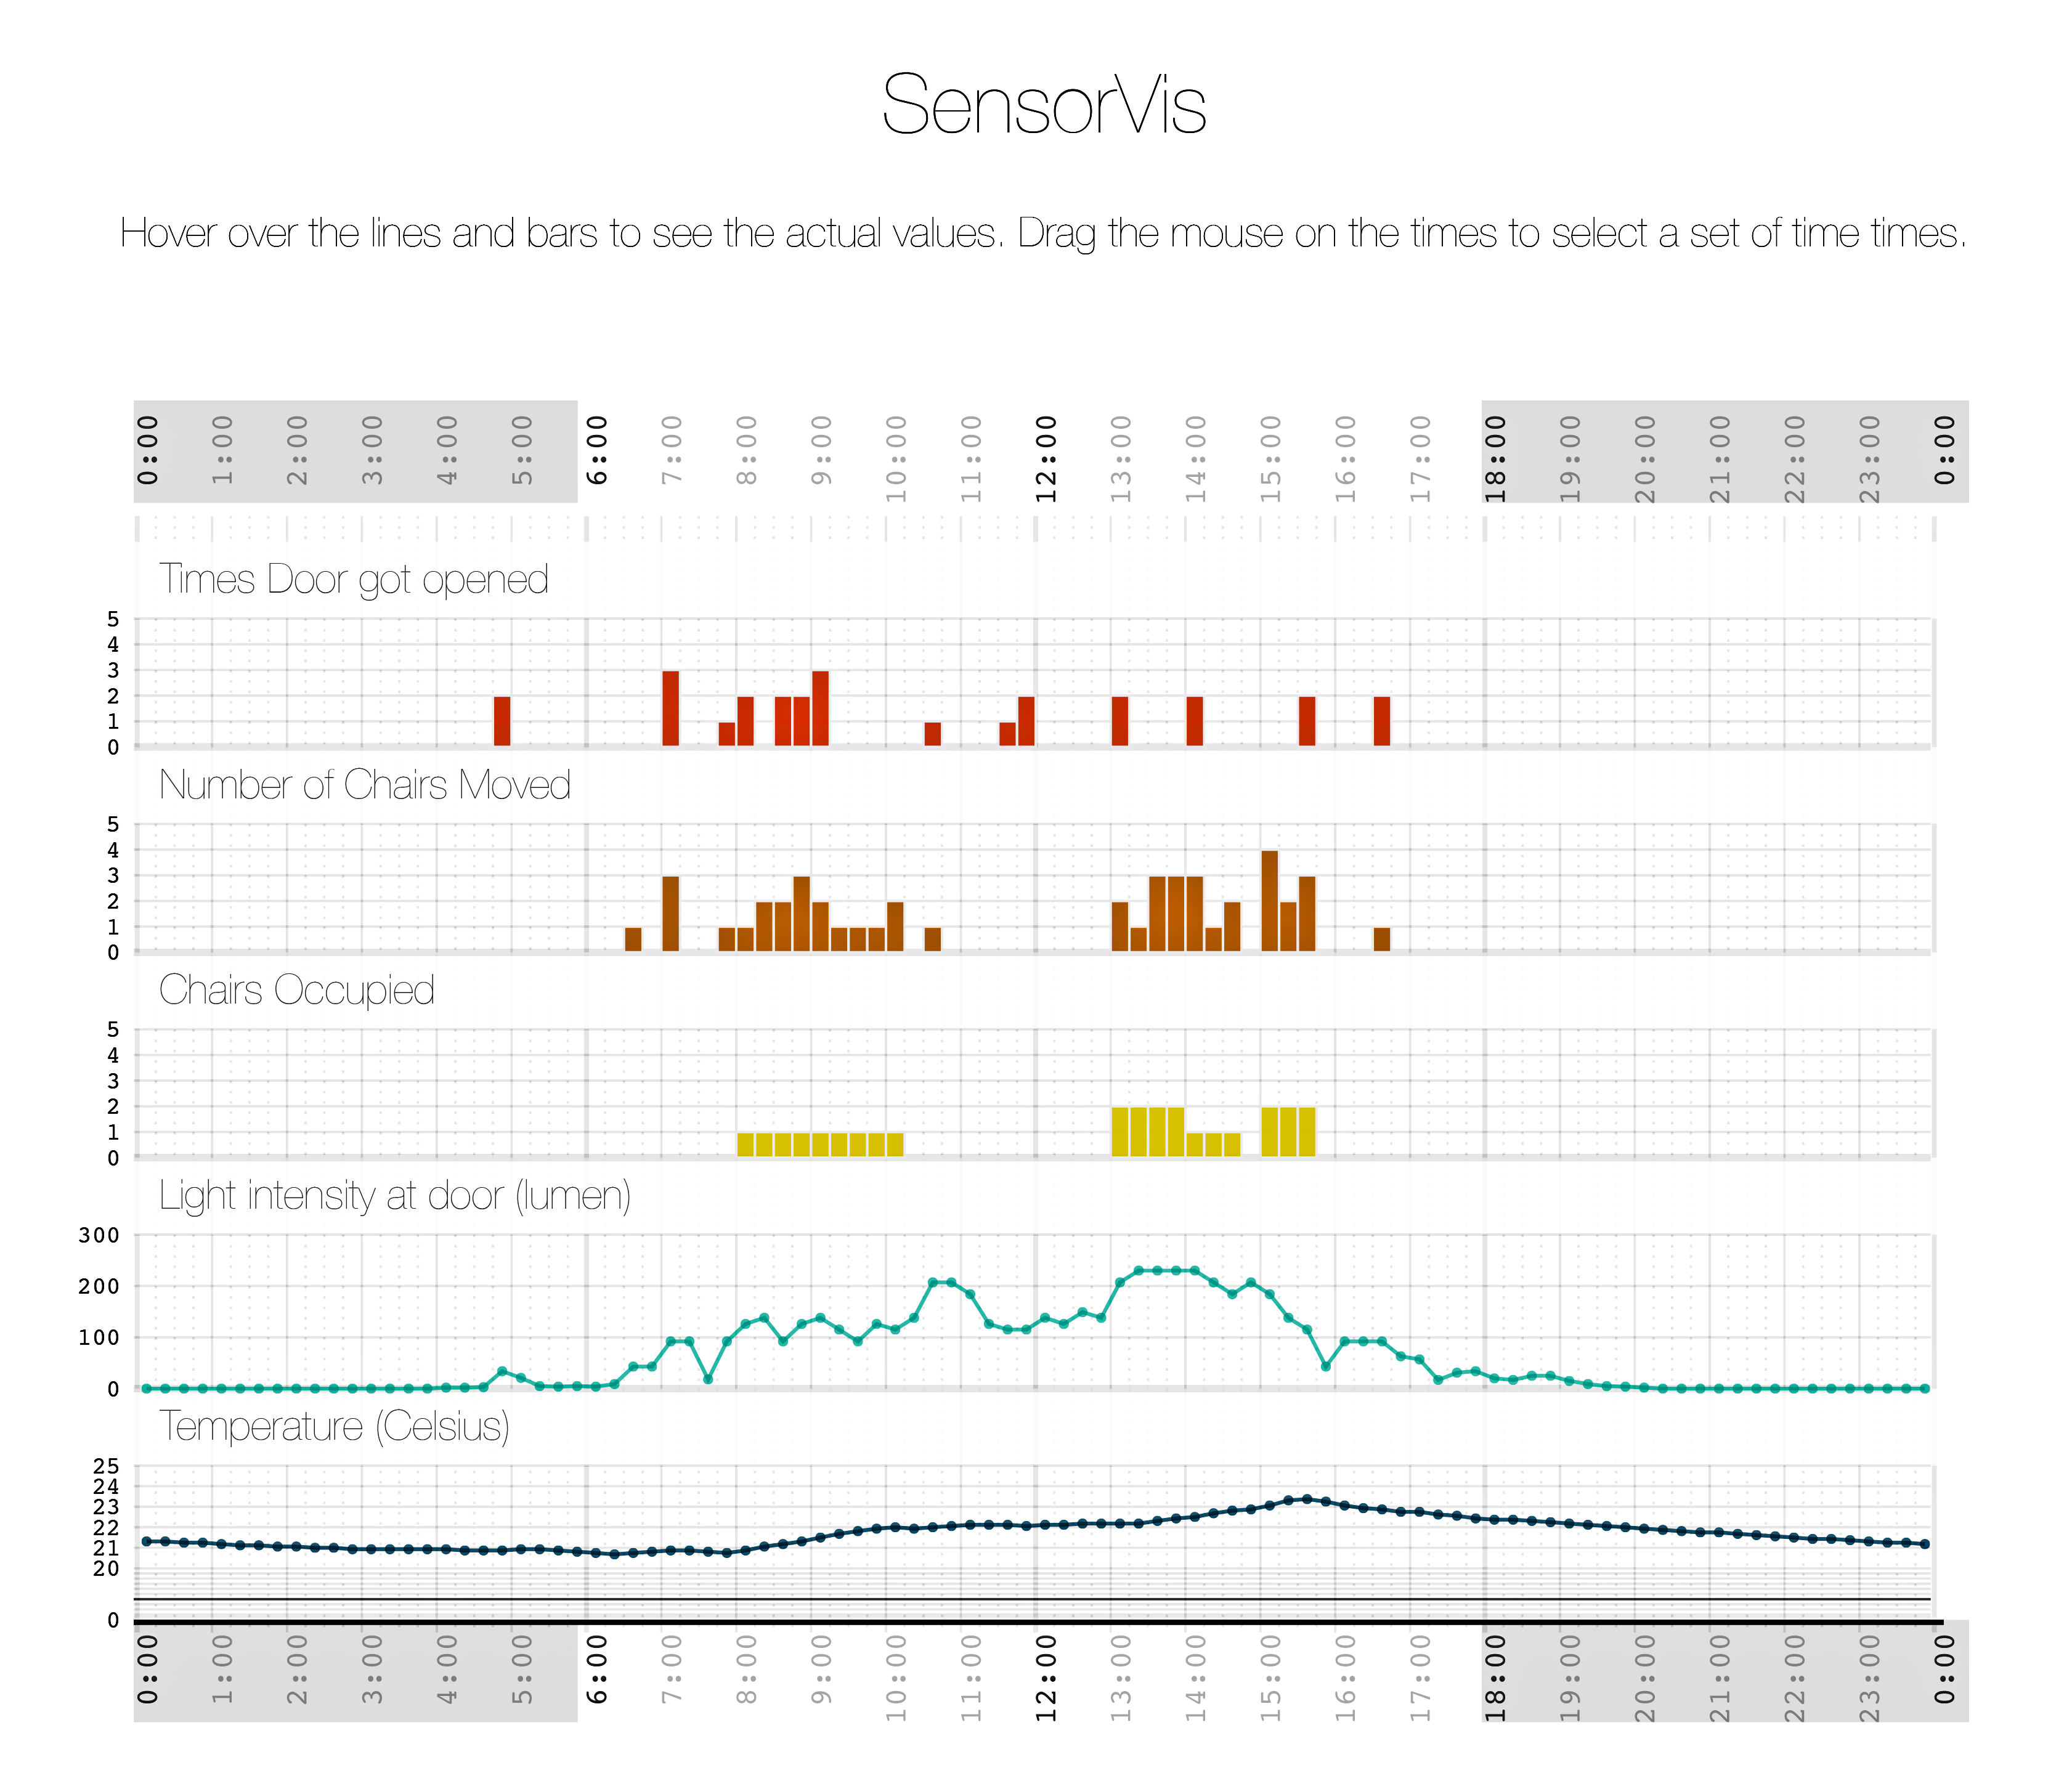
\includegraphics[scale=0.25]{images/occupancy.png}
  \caption{Screen dump of interactive data visualisation for a
    specific day. The $x$ axis shows the time dimension at 15 minute
    intervals over the course of the day. Horizontal bands show values
    for:  number of times the
    door was opened; the number of chairs that were moved; the number
    of the chairs that were occupied; the light intensity in the room
    in lumens; and the temperature of the room in degrees Celsius.}
  \label{fig:dataviz}
\end{figure}


We adapted the interviews (but not the focus groups) slightly from our
original plan to include a simple data visualisation. We asked
participants to `interpret’ the data visualisation. We also asked them
whether making the monitoring data public through data visualisation
might have an impact on people’s perceptions of the monitoring and on
their ability and interest to engage with the monitoring project.

\subsection{Participant Recruitment}
\label{sec:recruitment}

We recruited staff in Information Services who were based in Argyle
House, where the monitoring pilot was installed. An email from an IT
director was sent to all staff inviting them to participate (see
Appendix). A separate email was sent to managers in divisions to
highlight the project and ask them to encourage their staff to engage.
Due to low initial response, additional reminders were sent out.

We confirmed nine interview participants and six focus group participants,
divided into a group of two and a group of four, based on availability. One
of the interviewees was the head of facilities management; some of the
others had heard of the monitoring project and one had seen it come
through a security review, but otherwise none of them were directly
involved with it. Four interview participants were female and five
were male. Four focus group participants were female and two were
male. We did not ask people’s ages, but a general estimate is that
most participants were between 30 and 50 years of age.

\subsection{Data Analysis}
\label{sec:data-analysis}


Interviews were recorded, and the transcriptions and hand-written
notes were used to analyse the data. 

%%% Local Variables: ***
%%% mode:latex ***
%%% TeX-master: "main.tex"  ***
%%% End: ***